\section{Общ вид на алгоритъм за намиране на фрактал в $\mathbb{C}$}
\begin{Large}
Първо да отбележим, че компютърът само може да приближи фрактално множество, но не и да го намери точно.Обаче това не е проблем, ако се цели главно естетиката на полученото изображение. Обикновено се постъпва по следният начин за създаване на изображение:
\begin{enumerate}
\item На всеки пиксел се съпоставя число в комплексната равнина. Тъй като компютърните изображения са с правоъгълни измерения се съпоставят точки от даден правоъгълник в комплексната равнина. "Наслагвайки" растера върху правоъгълника получаваме множество от правоъгълни подобласти, като на всеки пиксел отговаря точка от съответния му регион. Обикновено се избира центърът, но ако желаем можем и горен,ляв край или друга точка.

\hspace{3cm}
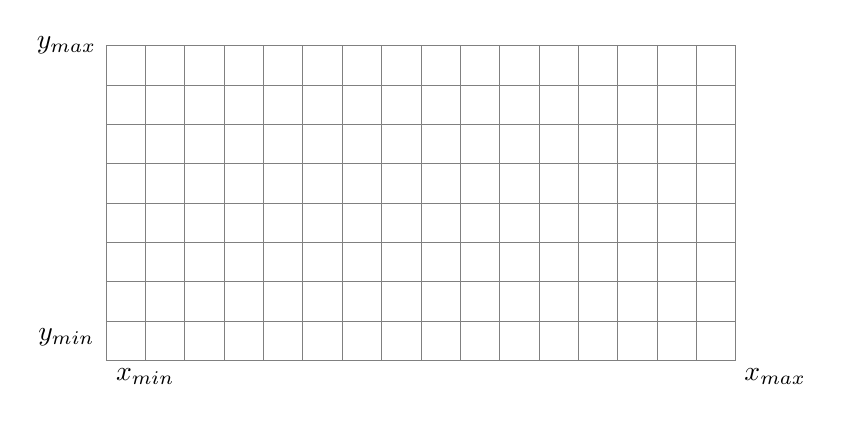
\begin{tikzpicture}

%\draw ++(0,0) -- ++(2,0) -- ++(0,-2) -- ++(-2,0)-- cycle;
%\draw ++(2,2) rectangle ++(3.5,-3.5);
\draw[step=0.5cm,gray,very thin] (0,0) grid (8,-4);
%\draw[step=1cm,red,very thin] (0.15,0.15) grid (7.85,-4.15);

\draw node at ++(0.5,-4.2) {$x_{min}$};
\draw node at ++(8.5,-4.2) {$x_{max}$};
\draw node at ++(-0.5,0) {$y_{max}$};
\draw node at ++(-0.5,-3.7) {$y_{min}$};
%\draw[very thick] (0,1) "point" -- (1,0);
%\draw \node at ++(0,0) "thick green point";
%\node {A} at (0,1) "ultra thick point";
%[anchor=south west]{$x_{min}$};
\end{tikzpicture}


\item За така определените точки се прилага многократно функцията $f(z)$ в цикъл. Цикълът продължава докато не е достигнат максимален определен брой итерации или достатъчно условие за неограниченост на нормите(затова и в много източници при изобазяване на \textfrak{M} това е $\left\Vert z_n \right\Vert > 2$).
\item В зависимост от типа на оцветяване:
\begin{itemize}
\item Итерацията се подава като аргумент на оцветяваща функция, която определя цвета на съответния пиксел.
\item Итерациите се запазват в масив. След приключване изчисленията за всички точки, цветът се определя по "нормирана" форма на итерацията, например разделятено на броя итерации за пиксела, върху общия брой на цялото изображение.
\end{itemize}
\item В зависимост от имплементацията, информацията за пикселите се запазва на момента от тяхното изчисление или след всички изчисления направо се запазва цялото изображение. 


\end{enumerate}

Ще отбележим, че такава е методологията и за създаване на фрактали от "Джулиев" тип.


\end{Large}